 %%%%%%%%%%%%%%%%%%%%%%%%
%% Sample use of the infthesis class to prepare a thesis. This can be used as 
%% a template to produce your own thesis.
%% 
%% The title, abstract and so on are taken from Martin Reddy's csthesis class
%% documentation.
%%
%% MEF, October 2002
%%%%%%%%%%%%%%%%%%%%%%%%

%% config the formatting
\documentclass[bsc,logo,plainprepages,parskip,abbrevs,10pt]{infthesis}

%% define the type of doc
\course{Software Engineering}
\project{Fourth Year Project Report}

%% import extra packages needed
%\usepackage{natbib}
\usepackage{url}
\usepackage{listings}
\usepackage{acronym}

%% information about the doc
\title{Design and Implemenation of a Low Power Wireless Medical Respirotory Network}
\author{Guy Taylor}
\submityear{2012}
\graduationdate{June 2012}

%% abstract
\abstract{
The Respire device provides low-power, unobtrusive respiratory monitoring of patients by use of
accelerometers to detect breathing movements. Implementation of a wireless networking capability
for this device will facilitate its widespread use in diagnosis and clinical management of respiratory
disease. The aim of this project was to develop Respire network firmware based on the \acf{TDMA}
method of network channel access, which was concluded to be the
only large-network (\textgreater 6 device constraint of the Respire hardware) method suitable for the Respire. I
produced and tested operational and debugging firmware for project development, which led to
identification of problems implementing TDMA with the Send-Receive function of the low-power
nRF24 radio onboard the Respire device. This has precluded testing of my design with the Respire
devices in a large-network environment. An important aspect of firmware development was to
include power-saving features where possible (\eg x\% reduction in power use when implementing
delays relative to code provided by the manufacturer). The project material (firmware, debugging
and testing systems) provides a basis for future development and application of the Respire family of
devices.
}

%% Now we start with the actual document.
\begin{document}

\begin{acronym}
\acro{TDMA}[TDMA]{Time Division Multiple Access}
\acro{ECG}[ECG]{Electrocardiogram}
\end{acronym}

%% First, the preliminary pages
\begin{preliminary}

%% This creates the title page
\maketitle

%% Acknowledgements
\begin{acknowledgements}
  Todo
\end{acknowledgements}

%% Next we need to have the declaration.
\standarddeclaration

%% Create the table of contents
\tableofcontents

%% If you want a list of figures or tables, uncomment the appropriate line(s)
\listoffigures
\listoftables

\end{preliminary}

%%%%%%%%
%% Include your chapter files here. See the sample chapter file for the basic
%% format.

%%
%% Copyright Guy Taylor 2012
%%
%%

\chapter{Introduction}

\section{Introduction}

The concept of medical equipment that enables unobtrusive wireless monitoring of various human
life-signs has been a recurring theme in science fiction for years\cite{StarTrekStarFleetTechnicalManual1986}, but only recently have
technological advancements been made that might help realize these possibilities and bring them to
market. Realizing the dream of detecting medical conditions early, even before they produce readily-detectable
symptoms, in people fit or ill entails both continuous monitoring of all vital signs (such as
pulse, respiratory rate and temperature) and their analysis in relation to known conditions or
detection trends over the person’s life. This possibility has sparked initiatives such as a 10 million
dollar prize for a "Tricorder"\cite{XprizeHealth2012} and new research into ways of measuring and analysing vital
signs.


In order for the researchers and medical staff to fully achieve these aims, hardware designers and
programmers need to produce platforms that are unobtrusive, easy-to-use and of low cost. A new
generation of devices and technologies are being designed and perfected as part of the research
process to system development, incorporating features such as the latest generation of low-power
\ac{MCU} and wireless transceivers suitable both for patient-monitoring devices
and, in a broader context, for small  consumer-electronics fitness aids\cite{Jawbone2012, Fitbit2012}.

\begin{wrapfigure}{r}{0.5\textwidth}
  \vspace{-10pt}
  \begin{center}
    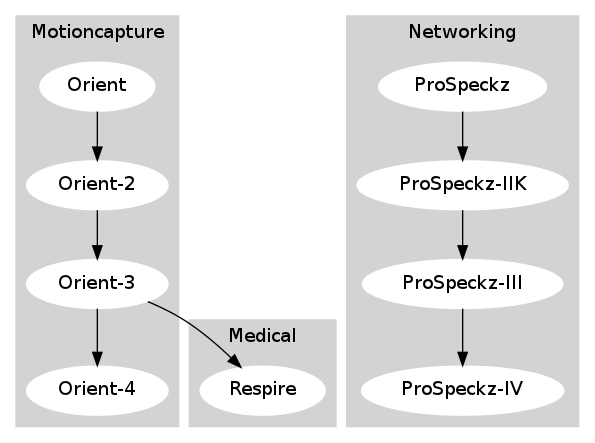
\includegraphics[width=0.4\textwidth, keepaspectratio=true]{images/respire_family_history.png}
  \end{center}
  \caption{Respire family history}
  \vspace{-10pt}
\end{wrapfigure}

The Centre for Speckled Computing within the School of Informatics, University of
Edinburgh, has produced several generations of small low-power sensor platforms for use
in motion capture and general research. These Orient\cite{Orient2012} and ProSpeckz\cite{ProSpeckz2012} devices
have facilitated hardware development and research, embracing the rapid prototype
design methodology. Building on the success of research projects with these devices, it
became apparent that more specific versions were needed both to enable new research and to
reduce the limitations of such a generic platform. This requirement, linked to the rapid development
of suitable microelectronics, has led to the production of two new devices built in tandem. These are
(1)The Respire, a respiratory monitoring device inspired by the Orient-3 motion-capture platform
but built from the ground up for low-power in a smaller, lighter package and (2) the new Orient-5,
upgrading the Orient motion-capture series to the latest generation of technology.

\section{Respiratory Monitoring}

\begin{wrapfigure}{r}{0.3\textwidth}
  \vspace{-10pt}
  \begin{center}
    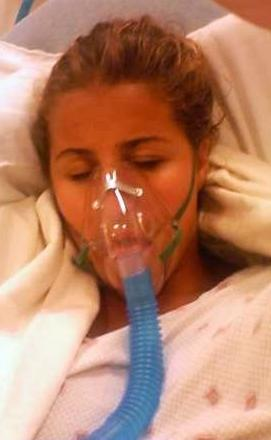
\includegraphics[width=0.2\textwidth, keepaspectratio=true]{images/Plastic_oxygen_mask_on_an_ER_patient.jpg}
  \end{center}
  \caption[Face Mask]{Face mask \cite{FaceMaskImg}}
  \vspace{-10pt}
\end{wrapfigure}

\subsection{Measurement of Respiratory Airflow}
At present the most effective and widely used systems for continuous respiratory monitoring in
people require the patient (or interested subjects) to wear a nasal cannula or face mask and directly
measure respiratory airflow. However, when not necessary for the medical administration of gasses,
these systems are both invasive and uncomfortable for the patient\cite{NasalCannula2011}. Whilst accurate, they
restrict patient movement and are unlikely to be used for long periods of time for monitoring alone.
It has however been demonstrated that an adaptation of the Respire accelerometer-based device
fitted to a nasal cannula could produce a workable wireless monitoring system.

\begin{wrapfigure}{l}{0.3\textwidth}
  \vspace{-10pt}
  \begin{center}
    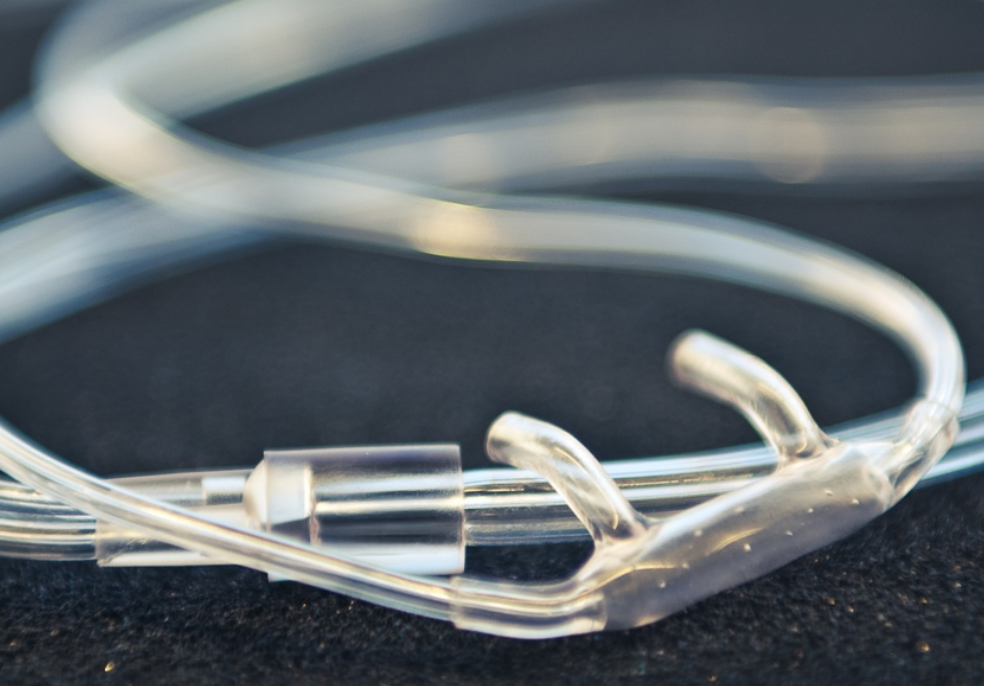
\includegraphics[width=0.2\textwidth, keepaspectratio=true]{images/nasal_canula.png}
  \end{center}
  \caption[Face Mask]{Nasal cannula \cite{SpecknetFlyer}}
  \vspace{-10pt}
\end{wrapfigure}

\subsubsection{Diaphragm Rotation}
The correlation between the rotation of the diaphragm (as measured by acceleration) and the
respiratory rate was recently shown to be accurate enough for medical use by the University of
Edinburgh team who designed the Respire device \cite{BatesLingMannArvind2010}. This non-invasive
means to measure the respiratory rate is achieved by affixing a small accelerometer onto
the patient's lower chest.


\subsubsection{\acf{ECG}}
It is also been shown that single or multiple lead \ac{ECG} can give a reasonable indication of respiratory
frequency ($\pm4$ breaths a minute) and is more independent of the wearer's movements than
accelerometers \cite{ZhaoZhaoQun2008, BoyleBidargaddiSarelaKarunanithi2009}.

\subsection{Usages}
Currently the main use of continuous respiratory monitoring is in intensive
care wards. In respiratory wards there is mainly only the use of non-continuous
60-second breath count measurements with the noting of breathing depth only in vague
terms \cite{Hunter2008}. It however is an increasing field of study, as with the availability of continuous measuring
devices, new diagnostics can be found. This mirrors the previous evolution of other medical
monitoring devices such as heart rate monitors and blood glucose analyzers.
% TODO (COPD ?) %
An example of the potential diagnostic power and applications of continuous respiratory
monitoring is in Sleep Apnoea. With real-time data collection, professionals can quickly diagnose the
condition whilst the patients can be alerted of their onset, thus preventing harm by waking up (ref). % TODO
For this to be successful the system must be unobtrusive enough to
sleep with and be reliable enough to be life-critical.
The overall goal of this project is to support the role of the medical
professionals and research staff in their attempts to find more
effective, comfortable and cheaper ways to diagnose and manage
respiratory conditions. To this end, the devices and designs are there specifically to enable this
purpose and not to break ground in other areas.
To enable collection of continuous respiratory rates, a device that can record and transmit
respiratory data wirelessly whilst still being small and light enough to be carried by the patient is
required. The device should be unobtrusive and simple to use, whilst decreasing the complexity of
the current system. This device should be suitable for use in hospitals at the required technical and
hygiene standards, in an environment that may contain multiple Respire devices and other
electronically controlled systems

\section{Goal}
This project proposes one solution for a new low power radio interface for the Respire device to
facilitate the more general use in a clinical setting.



%%
%% Copyright Guy Taylor 2012
%%
%%
\chapter{Discussion}

\section{The Respire radio}
The \ac{NRF24} radio was chosen for the Respire due to its low power utilisation
and its reduced complexity compared with competitors. Unfortunately for my specific
requirements in implementing \ac{TDMA}, the latter advantage was found to hinder
development. As a result of its basic interface it proved difficult to diagnose
apparent problems with the radio through a lack of status information and the
inability to easily monitor any radio communications.


As a result of this unforeseen project issue, significantly more time was spent
troubleshooting during development, thus reducing the time available to produce
an analysis of the network design. In hindsight, implementation of a non \ac{TDMA}
network (mainly \ac{FDMA} as it is still suitable for larger networks) would
circumvent the requirement for a final resolution of the discussed \ac{TDMA}
issue (section x). This alternative network design using \ac{FDMA}, although less
efficient, would have allowed the project to progress into the analysis of power
and network efficiency, not achieved in this project. This data would have then
allowed a cost-benefit analysis of additional complexity caused by a larger network
implementation. This would have allowed a discussion into the feasibility of
further development of this approach in later Respire versions.


My original approach to the implementation of the project was based around my
previous work with a sister device with a similar aim. More specifically, a
wireless sensor network using the ProSpeckz IIK, containing a CC2420 IEEE 802.15.4
radio configuration resembling that found in the Respire. This experience however,
was not sufficient to address the challenges impeding the progress of this project,
leading me to assume that the source of the difficulty lay out-with my implementation.
Of course, it is dangerous to assume that one's implementation is not flawed, so
with this in mind, over the course of the project, I designed several strategies
to isolate any possible issues. Working to a design methodology which promotes
reusability, I have outlined some of the relevant strategies below so that they
might be used to inform future development:
\begin{description}
  \item[\ac{NRF24} -- \ac{MCU} Communication Monitoring] \hfill \\
    Utilising an Open Bench Logic Sniffer digital probe (section {4.1.4}) to
    monitor the shared pins between the \ac{MCU} and radio was used throughout the
    project to validate firmware. Vital to the correct working of the \ac{NRF24} is
    both the correct configuration of its registers and accurate timing (in both
    communications and signalling). To address issues that arose during the first
    half of the project an effective methodology to measure and analyse the probe's
    data was developed. It was found that continuous analysis of the probe traces
    is key to effective testing in this situation. This continuous testing allowed
    changes with adverse effects, which may even not yet be noticed, to be identified
    and rectified early.
    
    An additional hardware circuit (section x) was used in a strategy to originally
    test if the \ac{LETIMER} was causing unknown signalling problems when a state is
    forced by direct \ac{GPIO} control. A secondary pin's signal was merged and
    monitored confirming this was not causing the issue being tested. Further use
    of this on other multiuse pins showed however that the \ac{SPI} \ac{CS} pin
    produced glitches when manually controlled whilst routed to the \ac{SPI},
    this was then simply fixed. As this circuit allowed multiple devices to be
    probed accurately at the same time it was utilised at the end of the project
    to allow accurate timing of transmissions.
  
  \item[Serial Console Printing via \ac{SWO}] \hfill \\
    As \ac{TDMA} and the radio itself is highly sensitive to timing constraints
    it was found single-stepping or break-point debugging produces its own effects
    on the results. To enable good debugging whilst maintaining normal code flow
    the \ac{SWO} pin was utilised. This was further simplified by adapting Newlib
    to support the use of \ac{SWO} through printf. (section {4.1.3})
  
  \item[Modular Testing] \hfill \\
    To identify if ``Standby-II'' state within the \ac{NRF24} was causing the issue
    (ref) in radio communications, or any other, many strategies where devised.
    By utilising the modular system, many rapid prototypes of solutions could be
    produced including: transmit and receive only solutions, ping-pong transfers,
    shortened chip enable periods, and \ac{MCU} only radio control. The results
    of these test demonstrated that there was an issue with transitioning between
    receive and transmit states however several other tests demonstrated the source
    of the problem due to a ``Standby-II'' state where proven to be inconclusive.
  
  \item[Hardware Testing] \hfill \\
    Utilising specialised spectrum analysers in the Dept of Informatics at
    Edinburgh University, the \ac{NRF24} test radios where placed into unmodulated
    carrier signal mode, the manufacturer's recommended testing method
    (Ref Constant carrier wave output for testing). None were found to be defective,
    removing the probability of defective hardware. This testing is combined with
    multiple use of all hardware (2xdevelopment board and 4xradio) during normal
    development.
  
  \item[Radio ``Sniffing''] \hfill \\
    I attempted to monitor radio communications both through the use of an
    Ubertooth spectrum analyser  in the addition to production of a radio sniffer
    using an \ac{NRF24} linked to a FTDI \ac{MPSSE}. Neither of these attempts 
    was able to detect \ac{NRF24} radio signals under any conditions, this is most
    likely due to the operation outside the devices specifications combined with
    unusual \ac{PHY} radio layer. However this should be further looked at as the
    ability to monitor radio traffic ``in the air'' would vastly improve troubleshooting.
\end{description}

Unfortunately the \ac{NRF24} radio is a fixed component of the Respire and could
not be replaced for testing of alternative radios. Therefore in my opinion, in order
for \ac{TDMA} to be applied successfully to a Respire network these problems with
the \ac{NRF24} will have to be overcome. This has recently become a greater priority
for the Respire section of the Speckled Computing group at Edinburgh University
because they are reaching the limitations of the simpler type of wireless system
currently in use.  I hope that this document detailing the issues around \ac{TDMA}
with the \ac{NRF24} will be of use to further developing the Respire and other
\ac{NRF24} products.

External to Edinburgh University, the \ac{NRF24} radio is currently used principally for use in wireless
keyboards and mice, with a maximum of 6 devices in each network. The recent family of Logitech
Unifying\textregistered devices, which allows these devices to to communicate with a single \ac{USB}
dongle, is one of the \ac{NRF24}'s largest known implementation. Within this type of configuration, devices do not need
to transition between transmit and receive states often and do not require synchronisation. I am
aware of two articles reporting successful implementation of a TDMA-based wireless sensor network
using the \ac{NRF24} family of radios \cite{GossipingMAC, DecentralizedTDMA} in other devices, which suggest that it should be possible to
use it within the requirements of the Respire project. From the information included in these
publications, I could not identify any significant differences between their approach and mine to
programming the \ac{NRF24}, although in both papers the NRF24L01 was used where as the Respire
contains the NRF24L01+. The stated difference between these two generations of \ac{NRF24} is that the
Respire version includes several hardware-accelerated networking features. I tested my system with
these features both enabled and disabled without any improvement.

\section{The Respire MCU}
The EFM32 appears to be an excellent choice for the Respire which, although not fully utilised in this
project, enables substantial power and lower energy improvements over the previous generations of
hardware. The consistency of the EMF32's pin configurations throughout its family of chipsalso
allows the MCU in the Respire to be replaced without need for a redesigned circuit board. This was
an an active design choice, as it allows the future Respire to use the EFM32 Cortex-M4, soon-to-be-
released, again reducing energy needs whilst improving performance by use ofa hardware floating-
point unit. This design to enable future change of EFM32 has again been used to reduce the time to
market by both allowing the immediate use of the Cortex-M3 line, with knowledge of the later
compatibility, and by using a more powerful chip allowing over time with optimisations lower power
replacements. I would of wished this design desision had also extended towards the radio circuitry.

%\section{Power Reductions}
%By Utilising the low-powe 32Khz clock on the EFM32 my design tried aimed to provide minumin MCU
%interation during the radio prosses. ...
%About the code in the respire that reduces it power in general and aid development
%Accuracy of the packet transmission time estimates

\section{Wireless Medical Devices and their Standardisation}

\subsection{Wireless Medical Device Standards}
At current there is no single standard for wireless medical equipment with many current viable
solutions. With each solution developed by competing organisations there is little sign that this
situation will change within the scope of the Respire project. It is however important when choosing
or developing a solution to review and analyse the competition.

\subsection{Bluetooth Lower Power}
The Bluetooth Special Interest Group and its Bluetooth standard is one of the most prevalent
Personal Area Networks (PAN) technologies. The next generation of the Bluetooth specification
includes a new Bluetooth Low Energy (BLE) sub-specification, specifically designed to address the
needs of sensor networks. BLE markedly reduces the power requirements for Frequency-hopping
spread spectrum that is prevalent in the full Bluetooth specification. BLE however has only just
become available with the recent finalisation of the standard, but it would be the most likely
alternative solution for the Respire.


\subsection{IEEE 802.15.4}
IEEE 802.15.4 provides a specification on many areas of a full wireless network, ranging from the
physical layer to the data to be sent over it. The broad approach of this specification has led to the
ZigBee standard, producing smaller more manageable standards to each application, including
health care. A second approach of managing the IEEE 802.15.5 specification has been to overlay the
IPv6 specification to produce 6LowPan.


\subsection{ANT}
ANT is a fully proprietary radio and network implementation designed to simplify the production of
wireless health care devices. As a recent and closed system, few devices have been produced
utilising its technology.


\subsection{\acf{ISM} Bands}
With the finite usable frequency ranges available to all wireless radio devices, and those devices that
emit radio interference, there are restrictive licensing systems in place. Licensing systems are
independently run by each country or region, but from 1980 a movement began to identify a set of
frequency bands that could be used worldwide without a licence \cite{ISMGen}.
With the introduction of the unlicensed (but still heavily restricted) \ac{ISM} bands,
communication via modern wireless equipment became a
widely-available possibility. A key 2.4 GHz band became the most popular for consumer electronics
communications due to its high bandwidth, long range and ability to pass through internal walls. This
convergence of signals into a single small band, , has created a crowded environment which,
compounded by the use of microwave ovens and other interference devices, needs powerful and
creative communication algorithms to penetrate and be reliable. The NRF24 uses Gaussian
frequency-shift keying to optimise throughput but does little to avoid interference. However it has
been shown that a frequency-hopping system to reduce the susceptibility to interference can be
implemented on the NRF24. (ref)


%\section{Related Work}
%
%\subsection{Edinburgh University}
%Edinburgh University, under the leadership of J Mann, has also produced a separate implementation
%of a radio interface for the Respire. This implementation was designed with power efficiency as the
%only goal. To this end the system is designed such that the radio is only on, and only broadcasts
%when data needs to be sent. This system therefore produces the most efficient power solution that
%could be implemented on the device, ignoring optimisations of the design. The system also uses the
%hardware accelerated ShockBurst\textregistered and MultiCeiver\textregistered system designed by Nordic Semiconductors.
%With a brief of a fully managed network system suitable for hospital use, this design was decided not
%to be suitable.Also by the extended use of the NRF24.the design has underused the features of the
%EFM32. With the ability for asynchronously clocked serial transfer automated by and interrupts and
%managed by the DMA not been utilised a similar chip could have been used.
%
%\subsection{Alabama University}
%To do

\section{Future Work}
I an attempt to improve the systems lower use it was found that the SPI connection to the radio is
under utilised by the use of a single buffer. I attempted To fix this issue with the use of the double
buffer but was unsuccessful due to a hardware flaw in the EFM32 (ref needed), where if the double
buffer and single buffer are used in the same application it is not reflected in the status of the buffer
free register. The issue was not overcome by the prescribed fix as the initial issue absorbed the time
allocated for the feature and therefore would be a good candidate for improving the system's
energy use. A secondary, and preferred, final solution for longer transfers would be to enable the
DMA and fully enable the EFM32 to power down the entire length of the transfer. I decided that the
DMA solution was out with the time constraints afforded to this section of the project and therefore
would also be a key step in improving the system's energy usage.
As many people believe strongly in their privacy, especially when concerning their medical records, it
should be considered if cryptography should be implemented on the system. This feature should not
impose as big an effect on the energy efficiency as most devices as the EFM32 has hardware
accelerated encryption, however it does not include any acceleration for hashes.



%%
%% Copyright Guy Taylor 2012
%%
%%

\chapter{Conclusion}

Although this project did not produce a final complete networking solution for the Respire, it has
developed firmware and analysed important aspects of system design that future work can build
upon. In particular, it has identified the onboard \ac{NRF24} radio as a weak link in the system required
to effect this particular solution. The Respire network is an excellent concept for improving patient
management and care (and also conceivably as a future as a health/fitness aid) and \ac{TDMA} is a
preferred protocol for implementing this network. If one of the new generation of low-power radios
(\eg Bluetooth Low Energy) is a suitable replacement to the \ac{NRF24} as a Respire device
modification, then I am confident that the firmware, debugging protocols and hardware connections
I have developed during this project will greatly facilitate testing and implementation of these
devices in a Respire network.



%%%%%%%%
%% Any appendices should go here. The appendix files should look just like the
%% chapter files.
\appendix
\chapter{ToDo}

\section{ToDo}
\begin{itemize}
  \item makefile
  \item graph wireless time sync vs wired to show that the dirift is not bad
  \item JTAG 20pin to SWD adaptor
  \item http://ieeexplore.ieee.org/Xplore/login.jsp?url=http%3A%2F%2Fieeexplore.ieee.org%2Fiel5%2F5639116%2F5654845%2F05656550.pdf%3Farnumber%3D5656550&authDecision=-203
  \item https://github.com/kevinmehall/nRF24L01-buspirate
\end{itemize}

(If you're wondering what all this weirdness is, check out\\
\url{http://www.subterrane.com/loremipsum.shtml})

Morbi ultricies. Proin consequat. Praesent consequat nulla a mauris.
Vivamus tellus. 





%% Choose your favourite bibliography style here.
\bibliographystyle{apalike}

%% If you want the bibliography single-spaced (which is allowed), uncomment
%% the next line.
% \singlespace

%% Specify the bibliography file.
\bibliography{references}

%% ... that's all, folks!
\end{document}

